\chapter{Spectral Scale Selection for Kernel Density Estimation}

In this chapter, we apply the scale selection methodology from chapter~\ref{chap:intro_meth} to a sequence of kernel density estimates $\{\hat{f}_{h_i}\}_{i=1}^{N}$.

\section{Preliminaries on Kernel Density Estimation}

We have data $X_1,\dots.X_n\in\mathbb{R}^{d}$ sampled from an (unknown) distribution with density $f$. The kernel density function $\hat{f}_h$ estimates this unknown density. It is defined by
\begin{align*}
    \hat{f}_h(x)\coloneqq \frac{1}{nh^d}\sum_{j=1}^{n}K\left(\frac{x-X_j}{h}\right),\quad x\in\mathbb{R}^d.
\end{align*}

Two common choices for the kernel $K$ are:
\begin{itemize}
    \item the Epanechnikov kernel $K(u)=\mathbf{1}\{-1\le u\le1\}3(1-u^2)/4$
    \item the Gaussian kernel $K(u)=(2\pi)^{-1/2}\exp{(-u^2/2)}$
\end{itemize}

From now on, we always work with the Gaussian kernel, if not indicated otherwise.

The question of how to choose the bandwidth $h$ is widely known in the literature. See reviews~[]. We present some of the most popular methods below, which we also use to compare with our newly developed spectral selector. Following the review~\cite{heidenreich_bandwidth_2013}, bandwidth selectors can be divided into several classes, including plug-in and cross-validation methods. The methods of both classes minimize some approximation of the (mean) integrated squared error.

\begin{Def}
    Let $f$ be a density and $\hat{f}_h$ its kernel density estimate. The integrated squared error (ISE) between $f$ and $\hat{f}_h$ is given by
    \begin{align*}
        \operatorname{ISE}(h)\coloneqq \int\left(f(x)-\hat{f}_h(x)\right)^2\,dx.
    \end{align*}
    The mean integrated squared error (MISE) is $\operatorname{MISE}(h)\coloneqq\mathbb{E}[\operatorname{ISE}(h)]$.
\end{Def}



\subsection*{Cross-variance methods}

The ISE can be written as
\begin{align*}
    \operatorname{ISE}(h)=\int\hat{f}_h(x)^2\,dx-2\mathbb{E}_{X\sim f}\left[\hat{f}_h(X)\right]+\int f(x)^2\,dx
\end{align*}

The Ordinary Least Squares Cross-Variance estimator is given by
\begin{align*}
    \operatorname{CV}(h)=\int\hat{f}_h(x)\,dx-\frac{2}{n}\sum_{i=1}^{n}\hat{f}_{h,-i}(X_i),\quad\hat{h}_{\operatorname{CV}}\in\arg\min\operatorname{CV}(h)
\end{align*}
Here, $\hat{f}_{h,-i}$ is the kernel density function where the observation $X_i$ is left out, that is,
\begin{align*}
    \hat{f}_{h,-i}(x)=\frac{1}{(n-1)h}\sum_{j\ne i}K\left(\frac{x-X_j}{h}\right)
\end{align*}

\subsection*{Plug-in methods}

The bias-variance decomposition of the MISE is
\begin{align*}
    \operatorname{MISE}(h)=\int\operatorname{Var}[\hat{f}_h(x)]\,dx+\int\operatorname{Bias}(\hat{f}_h(x))\,dx
\end{align*}
with
\begin{align*}
    \operatorname{IV}(h)&=\int\operatorname{Var}[\hat{f}_h(x)]\,dx=\frac{\|K\|_2^2}{nh^{d}}-\frac{\|K_h\ast f\|_2^2}{n},\quad\text{and}\\
    \operatorname{ISB}(h)&=\int\operatorname{Bias}(\hat{f}_h(x))\,dx=\|K_h\ast f-f\|_2^2
\end{align*}

This decomposition gives conditions on $h=h_n$ so that the kernel density estimate $\hat{f}_{h_n}$ is consistent. Namely, it must hold $h_n\to0$ and $nh_n^d\to+\infty$. An example of such a sequence is $h_n=cn^{-\alpha}$ for some $c>0$ and $\alpha\in(0,1)$.

The MISE can be written as
\begin{align*}
    \operatorname{MISE}(h)=\underbrace{\frac{\|K\|_2^2}{nh}+\frac{h^4}{4}\mu_2(K)^2\|f^{''}\|_2^2}_{=\operatorname{AMISE}(h)}+o\left(\frac{1}{nh}+h^{4}\right)
\end{align*}

Minimizing the AMISE leads to
\begin{align}\label{eq:h_amise}
    h_{\operatorname{AMISE}}=\left(\frac{\|K\|_2^2}{n\mu_2(K)^2\|f^{''}\|_2^2}\right)^{1/5}
\end{align}

\todo[inline]{check for general dimension $d$}

The optimal bandwidth thus behaves like $n^{-1/5}$.

Plug-in methods use Equation~\eqref{eq:h_amise} as starting point. Silverman's rule of thumb assumes that $f$ is the density of a normal distribution $N(0,\sigma^2)$. In this case, $\|f^{''}\|_2^2$ can simply be computed and plugged into Equation~\eqref{eq:h_amise}:
\begin{align*}
    \|f^{''}\|_2^2=\frac{3}{8\sqrt{\pi}\sigma^{5}},\quad h_{\operatorname{AMISE}}=\left(\frac{4}{3}\right)^{1/5}\sigma n^{-1/5}\approx1.06\sigma n^{-1/5}
\end{align*}

\todo[inline]{introduce (improved) Sheather and Jones' plug in}

\subsection*{Exact MISE representation for Gaussian mixture model}

Exact computations are generally not possible since the true density $f$ of the sampled data $X_1,\dots,X_n$ is not known. In simulation experiments, of course, we simulate the data ourselves and thus know the density $f$. For certain choices of the true density $f$, explicit formulas for the MISE exist.


A particularly broad and well studied class is that of Gaussian mixture models. They are characterized by densities $f$ of the form $f=\sum_{l=1}^{L}w_l\phi_{m_l,\sigma_l^2}$, where $w_l>0$, $\sum_lw_l=1$, $m_l\in\mathbb{R}$, and $\sigma_l^2>0$.

Marron and Wand~\cite{10.1214/aos/1176348653} derive an explicit formula for the MISE between a density $f$ of the Gaussian mixture model and its kernel density estimate with Gaussian kernel of order $r\in\mathbb{N}$. Here we state the formula for the special case $r=1$, that is, for the standard Gaussian kernel.

\begin{Prop}
    The mean integrated squared error between a kernel density estimate $\hat{f}_h$ with Gaussian kernel and the density function $f$ of a Gaussian mixture model with weights $w_l$, variances $s_l^2$ and means $m_l$ is given by
    \begin{align*}
        \operatorname{MISE}(h)&=\frac{1}{2\sqrt{\pi}}\frac{1}{nh}+\left(1-\frac{1}{n}\right)\mathcal{K}(h,2)-2\mathcal{K}(h,1)+\mathcal{K}(h,0),\\
        \mathcal{K}(h,q)&=\sum_{l,l'=1}^{L}\frac{w_lw_{l'}}{\sqrt{s_l^2+s_{l'}^2+qh^2}}\phi\left(\frac{m_l-m_{l'}}{\sqrt{s_l^2+s_{l'}^2+qh^2}}\right),\quad q\in\{0,1,2\}.
    \end{align*}
\end{Prop}



Minimizing $\operatorname{MISE}(h)$ yields the \enquote{oracle} bandwidth $h_{\text{oracle}}$. We will use the oracle bandwidth as an ultimate benchmark in all settings where $\operatorname{MISE}$ has an explicit representation and thus can be minimized using standard methods.


\subsection*{Constructing Mixture Models with multiple global MISE minima}

\todo[inline]{Discuss uniqueness of MISE curve for Gaussian mixture models}



Since the optimal bandwidth minimizes the MISE, particularly interesting scenarios arise in cases where the MISE has no unique minimum. 

Since for Gaussian kernels and Gaussian mixture densities the mean integrated squared error has a closed form, we can find $w_l$, $m_l$, $s_l^2$ such that there exist $h_1<h_2$ that are both global minima of the MISE curve.

\todo[inline]{add construction principle and example, there are different classes of local minima pairs}

This serves as an easy example of a situation where the optimal bandwidth is not unique and thus is a particularly interesting test for spectrally selected bandwidths.

Figure~\ref{fig:equal-minima-example} illustrates a Gaussian mixture density with two local MISE minima.

\begin{figure}[htbp]
    \centering
    \begin{subfigure}{0.48\textwidth}
        \centering
        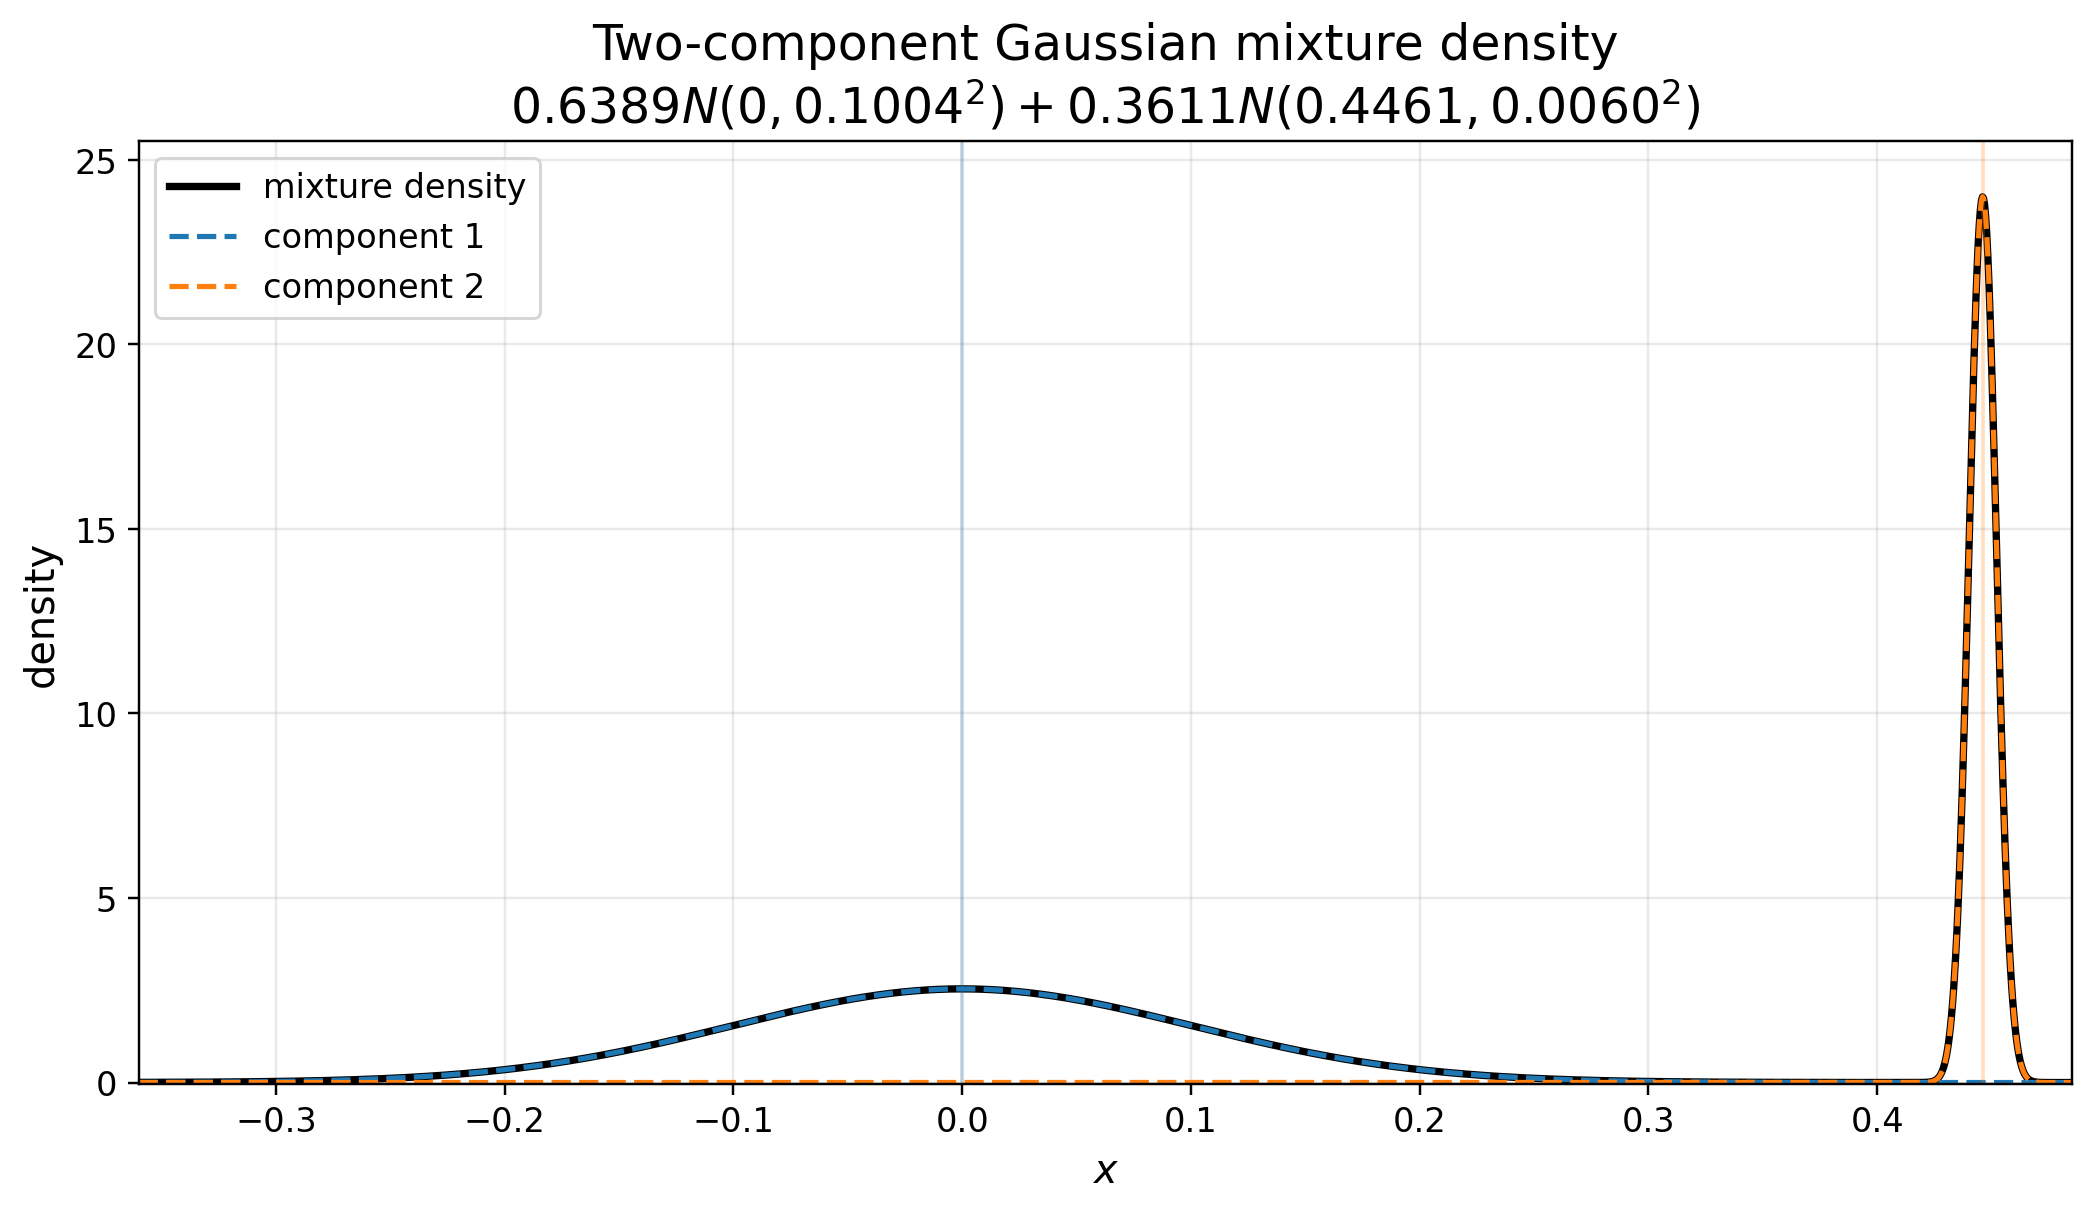
\includegraphics[width=\linewidth]{Code/Code_kde/outputs/equal_minima_mixture_pdf_clean.png}
        \caption{Gaussian mixture density.}
        \label{fig:equal-minima-density}
    \end{subfigure}
    \hfill
    \begin{subfigure}{0.48\textwidth}
        \centering
        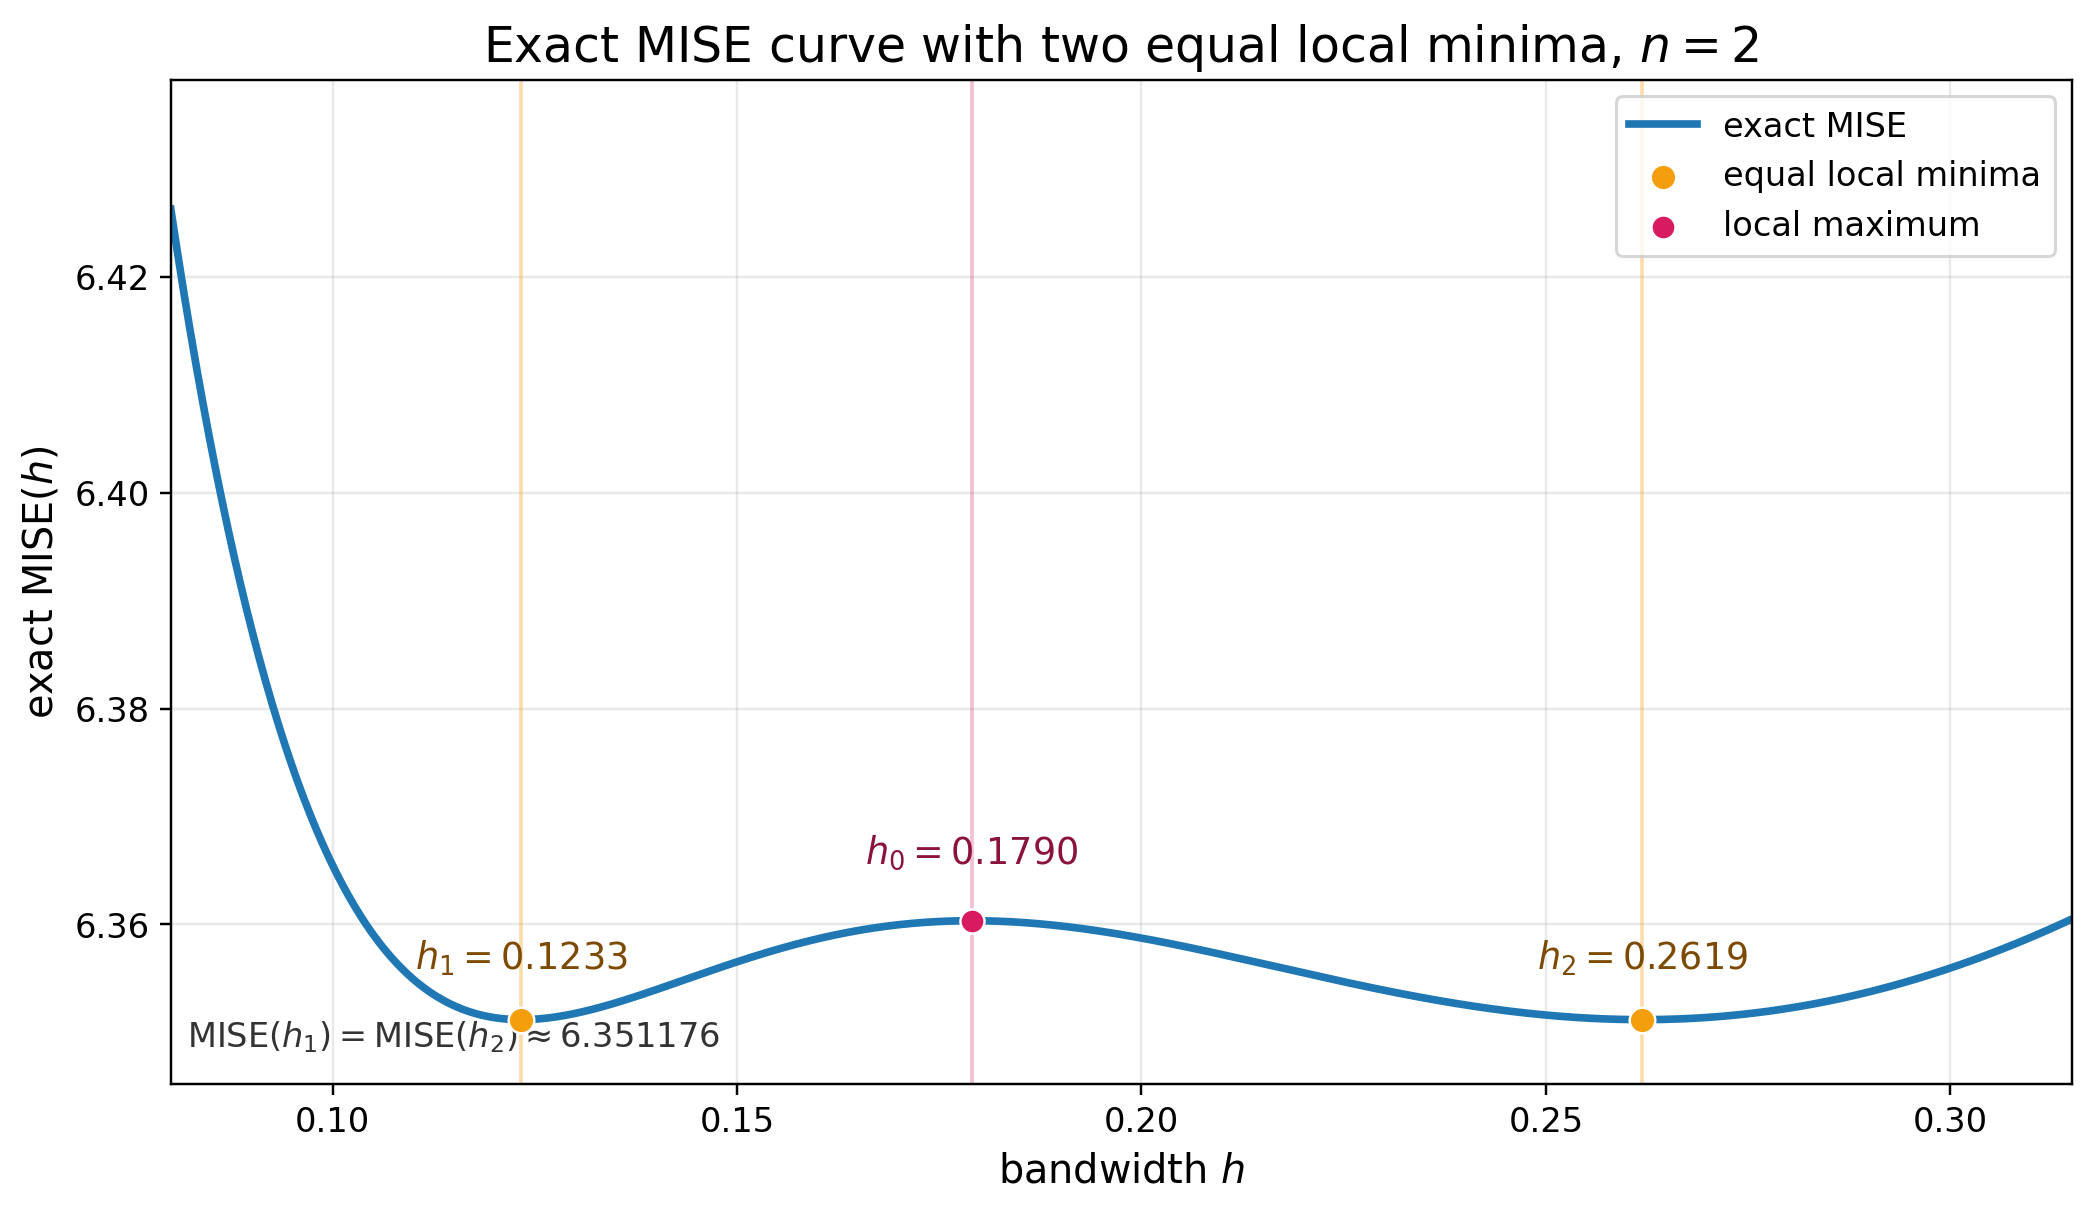
\includegraphics[width=\linewidth]{Code/Code_kde/outputs/mise_equal_minima_constructed.png}
        \caption{Exact MISE curve.}
        \label{fig:equal-minima-mise}
    \end{subfigure}

    \caption{Example of a Gaussian mixture density whose exact MISE curve has two equal local minima.}
    \label{fig:equal-minima-example}
\end{figure}

\section{Divergences between distributions}

\todo[inline]{Introduce the general definition that uses manifolds}

We follow the survey~\cite{nielsen_elementary_2020}.

Let $\mathcal{P}$ be the set of all absolutely continuous probability distributions on $(\mathbb{R}^d,\mathcal{B}(\mathbb{R}^d))$. That is,
\begin{align*}
    \mathcal{P}=\{\mu:\exists f:\mathbb{R}\to\mathbb{R}\text{ measurable},f\ge0,\mu(F)=\int_Ff\,d\lambda\}
\end{align*}

A divergence is a map $D:\mathcal{P}\times\mathcal{P}\to\mathbb{R}_{\ge0}$ such that $D(p,q)=0$ if and only if $p=q$.

The two most important classes of divergences are $f$-divergences and Bregman divergences.

\subsection{\texorpdfstring{$f$}{f}-divergences}

\subsubsection*{Definition and Motivation}

\todo[inline]{Connect $f$-divergence to generalized entropy}

Let $f:\mathbb{R}_{\ge0}\to\mathbb{R}\cup\{+\infty\}$ be a convex function. The $f$-divergence is defined as
\begin{align*}
    D_f(p\|q)=\int f\left(\frac{p(x)}{q(x)}\right)q(x)\,dx
\end{align*}

The $f$-divergence is symmetric iff $f(t)=tf(1/t)+c(t-1)$ for some constant $c$. In particular, the $\alpha$-divergence is symmetric iff $\alpha=1/2$ (Hellinger distance). The only symmetric $\chi^{\alpha}$-divergence is the total variation distance. The JS-divergence is also symmetric.

\todo[inline]{Cite or prove the symmetry characterization}

\subsubsection*{Amari alpha divergence}

A prominent parametrized family of $f$-divergences is the so called $\alpha$-divergence (see \cite{cichocki_families_2010}) where the function $f=f_{\alpha}$ is given by
\begin{align*}
    f_{\alpha}(t)=\frac{1}{\alpha(\alpha-1)}\left(t^{\alpha}-\alpha t-(1-\alpha)\right)
\end{align*}
The actual divergence is then given by
\begin{align*}
    D_{\alpha}(p\|q)=\frac{1}{\alpha(\alpha-1)}\left(\int p(x)^{\alpha}q(x)^{1-\alpha}\,dx-1\right)
\end{align*}

By taking the limit $\alpha\to1$ we recover the Kullback-Leibler divergence, whereas taking the limit $\alpha\to0$ recovers the reverse Kullback-Leibler divergence. At $\alpha=1/2$ we obtain $D_{1/2}(p\|q)=4D_H(p,q)$, where $D_H(p,q)=(1/2)\int(\sqrt{f}-\sqrt{g})^2$ is the squared Hellinger distance.

\todo[inline]{Mention two different parameterizations}

\subsubsection*{chi squared divergence (total variance)}

Another class of divergences are the $\chi^{\alpha}$-divergences (see~[]). They are determined by $f_{\alpha}(t)=(1/2)|t-1|^{\alpha}$, where $\alpha\ge1$. Setting $\alpha=1$ recovers the well known total variation distance: $d_{\text{TV}}(p,q)=(1/2)\int|p-q|$.

\subsubsection*{JS divergence}

Another important divergence that belongs to the class of $f$-divergences is the Jensen Shannon divergence. The function $f$ is set to be
\begin{align*}
    f(t)=\frac{1}{2}\left(t\log{t}-(t+1)\log{\frac{t+1}{2}}\right)
\end{align*}
The divergence is then given by
\begin{align*}
    \operatorname{JS}(f,g)=H\left(\frac{f+g}{2}\right)-\frac{1}{2}H(f)-\frac{1}{2}H(g),
\end{align*}
where $H(f)=-\int f\log{f}$ is the Shannon entropy.

\subsubsection*{Renyi divergence}

The class of Rényi divergences is defined as
\begin{align*}
    R_{\alpha}(p\|q)=\frac{1}{\alpha-1}\log{\left(\int p(x)^{\alpha}q(x)^{1-\alpha}\,dx\right)},
\end{align*}
where $\alpha\in\mathbb{R}\setminus\{1\}$ is the order. In case of $\alpha>1$, we read $f^{\alpha}g^{1-\alpha}=f^{\alpha}/g^{\alpha-1}$. The limiting case $\alpha\to1$ recovers the Kullback-Leibler divergence.

The Rény divergence and the $\alpha$-divergence are different transformations of the same integral $C_{\alpha}(p,q)=\int p^{\alpha}q^{1-\alpha}$. We have
\begin{align*}
    R_{\alpha}(p\|q)&=g(C_{\alpha}(p,q)),\quad g(t)=\frac{1}{\alpha-1}\log{t}\\
    D_{\alpha}(p\|q)&=h(C_{\alpha}(p,q)),\quad h(t)=\frac{1}{\alpha(\alpha-1)}(t-1)
\end{align*}

\todo[inline]{transformations in each other}

By Hölders inequality $0\le C_{\alpha}(p,q)\le 1$.

\subsection{Bregman divergences}

The second major class are Bregman divergences, which are defined by
\begin{align*}
    D_F(p\| q)=F(p)-F(q)-\langle\nabla F(q),p-q\rangle,
\end{align*}
where $F\in C^{1}$. A particular subclass is given by
\begin{align*}
    F_{\phi}(p)=\int\phi(p(x))\,dx
\end{align*}
for some convex function $\phi$. An example of such a function $\phi$ is the class of $\beta$-divergences determined by
\begin{align*}
    \phi_{\beta}(t)=\frac{t^{1+\beta}}{\beta(\beta+1)},\quad\beta\in\mathbb{R}\setminus\{0,-1\}
\end{align*}

\todo[inline]{Condition on $F$ or $\phi$ under which Bregman divergence is symmetric}

The $\beta$-divergence is thus given by
\begin{align*}
    D_{\beta}(p,q)=\frac{1}{\beta(\beta-1)}\left(\int p^{\beta}+(\beta-1)\int q^{\beta}-\beta\int pq^{\beta-1}\right)
\end{align*}

For $\beta=2$ we get
\begin{align*}
    D_2(p,q)=\frac{1}{2}\int(p-q)^2=\frac{1}{2}\|p-q\|_2^2
\end{align*}

If $p(x)=\hat{f}_h(x)=n^{-1}\sum_jK_h(x-X_j)$ and $q(x)=\hat{f}_s(x)=n^{-1}\sum_jK_h(x-X_j)$ are kernel density estimates with a Gaussian kernel $K$, we can obtain an explicit formula for $D_2(\hat{f}_h,\hat{f}_s)$. We have
\begin{align}\label{eq:exact_l2_divergence}
    D_2(\hat{f}_h,\hat{f}_s)=\frac{1}{2n^2}\sum_{i,j}\left(\phi_{\sqrt{2}h}(X_i-X_j)+\phi_{\sqrt{2}s}(X_i-X_j)-\phi_{\sqrt{h^2+s^2}}(X_i-X_j)\right)
\end{align}
The derivation of the formula uses mainly the Gaussian convolution identity, that is, the fact that for Gaussian densities $f_1=\phi_{\mu_1,\sigma_1^2}$ and $f_2=\phi_{\mu_2,\sigma_2^2}$ their convolution is $f_1\ast f_2=\phi_{\mu_1+\mu_2,\sigma_1^2+\sigma_2^2}$.

\subsubsection*{Relations between all presented divergences}

\todo[inline]{Do all these divergences relate to each other?}

\begin{Prop}
    Let $D$ be a divergence such that it is a $f$-divergence for some $f$ and simultaneously a Bregman divergence for some $F$. This is sufficient and necessary for $D$ to be the Kullback-Leibler divergence.
\end{Prop}

\section{Assembly of Scale Similarity Matrices}

A matrix $A\in\mathbb{R}^{n\times n}$ is positive definite if $x^TAx>0$ for all $x\in\mathbb{R}^n$, $x\ne0$. A symmetric map $D:X\times X\to\mathbb{R}$ with $D(x,x)=0$ is called conditionally negative definite if
\begin{align*}
    \sum_{i,j=1}^{n}a_ia_jD(x_i,x_j)\le0
\end{align*}
for all $x_1,\dots,x_n\in X$ and $a_1,\dots,a_n\in\mathbb{R}$ with $\sum_{i}a_i=0$. A function $\phi:(0.\infty)\to\mathbb{R}$ is called completely monotone if $\phi\in C^{\infty}(0,\infty)$ and $(-1)^{n}\phi^{(n)}(t)\ge 0$ for all $n\in\mathbb{N}_0$ and $t>0$.

\todo[inline]{Which divergencies are conditionally negative definite and which not; Jensen Shannon? (Fuglede and Topsøe)}

The most prominent example of a completely monotone function is $\phi(t)=e^{-\gamma t^{\alpha}}$, $\gamma\ge0$, $0<\alpha\le1$.

\begin{Thm}[Schoenberg]\label{thm:schoenberg}
    Let $D:X\times X\to\mathbb{R}$ be conditionally negative. Let $x_1,\dots,x_n\in X$. If $\phi$ is completely monotone, then the matrix $\Sigma=(\Sigma_{ij})$, $\Sigma_{ij}=\phi(D(x_i,x_j))$ is positive definite.
    \todo[inline]{Find a source to cite}
\end{Thm}

\todo[inline]{connect to Bernstein–Widder}

Theorem~\ref{thm:schoenberg} gives a general construction principle for the scale similarity matrix $\Sigma^{(N)}=(\Sigma^{(N)}_{ij})$. Namely, we set $\Sigma^{(N)}_{ij}=\phi(D(\hat{f}_{h_i},\hat{f}_{h_j}))$ where $D$ is some divergence and $\phi$ a completely monotone function. 

There are some special kinds of divergences, where a transformation by a not necessarily completely monotone function is enough to obtain a positive definite similarity matrix.

\todo[inline]{What is it about these special divergences that do not require a completely monotone transformation?}

The transformation $S_{ij}=\exp{\{-D_{ij}/\tau\}}$ can be motivated as follows. Let $H(p)=-\sum_jp_j\log{p_j}$ be the entropy of the probability vector $p\in\mathbb{R}^{N}$. The quantity
\begin{align*}
    \sum_{j=1}^{N}p_jD_{ij}-\tau H(p)
\end{align*}
is minimized by $p_i=(p_{i1},\dots,p_{iN})$, where $p_{ij}=S_{ij}/\sum_{k=1}^{N}S_{ik}$. In that sense, $\tau$ can be interpreted as a penalty weight. This is another instance of the Donsker–Varadhan variational principle. See~\cite{anantharam_variational_2017} for reference.

Apply the transformation $\exp{(-\tau D_{\alpha})}$ to the Renyi divergence $D_{\alpha}$ yields
\begin{align*}
    S_{ij}&=\exp{(-\tau D_{\alpha}(\hat{f}_{h_i},\hat{f}_{h_j}))}\\
    &=\exp{\left\{\frac{\tau}{1-\alpha}\log{C_{\alpha}(\hat{f}_{h_i},\hat{f}_{h_j})}\right\}}\\
    &=C_{\alpha}(\hat{f}_{h_i},\hat{f}_{h_j})^{\frac{\tau}{1-\alpha}}
\end{align*}

\subsection*{Why not use the divergence matrix for spectral scale selection?}

In this subsection, we want to briefly give an argument why it is not advisable to compute the Perron vector of the divergence matrix $D$ itself and thus motivate the above similarity transformation more.

\begin{Def}[Robinson matrix]
    A matrix $D$ with entries $D_{ij}=D(x_i,x_j)$ is called a Robinson matrix (cf.~\cite{carmona_two_2024}) if there exists a permutation $\pi$ on $\{1,\dots,N\}$ such that for $D_{ij}^{\pi}=D(x_{\pi(i)},x_{\pi(j)})$ it holds
    \begin{align*}
        D^{\pi}_{ik}\ge\max\{D^{\pi}_{ij},D^{\pi}_{jk}\}\text{ and }D_{ki}^{\pi}\ge\max\{D_{ji}^{\pi},D_{kj}^{\pi}\}
    \end{align*}
    whenever $i<j<k$.
\end{Def}

\todo[inline]{Prove that for Gaussian kernels we obtain a Robinson matrix?}

The reason why we do not want to work with the matrix $D$ and instead transform to a similarity matrix $\phi(D)$ is due to the following Lemma.

\begin{Lem}
    Let $(M,d)$ be a geodesic metric space such that for every fixed point $y\in X$, the function $x\mapsto d(x,y)$ is geodesically convex. Let $X\subseteq M$ be a convex subset. Let $x_1,\dots,x_N\in X$ be finitely many points and define the distance matrix $D=(d(x_i,x_j))_{i,j=1}^{N}$. Let $v=(v_j)\in\mathbb{R}^{N}$ be the Perron vector of $D$. Then
    \begin{align*}
        \arg\max_{1\le j\le N}v_j\subseteq\{1,N\}.
    \end{align*}
    \todo[inline]{Find correct assumptions to prove the Lemma}
    \todo[inline]{This Lemma is not correct yet but numerical experiments suggest that the Perron vector of divergence matrices behaves not how we want}
\end{Lem}

\begin{proof}
    Define the function
    \begin{align*}
        F(x)=\sum_{j=1}^{N}d(x,x_j)v_j,\quad x\in X.
    \end{align*}
    Since $v$ is the Perron vector, we have $F(x_i)=\lambda v_i$. Thus
    \begin{align*}
        \arg\max_{1\le j\le N} v_j=\arg\max_{1\le j\le N}F(x_j).
    \end{align*}
\end{proof}

\subsection*{Approximating integrals using quadrature}

Computing divergences between densities amounts to evaluating integrals of the form $\int_{-\infty}^{+\infty}C_{\alpha}(p,q)$, where, for example, in the case of the $\alpha$ or Rényi divergence, $C_{\alpha}(p,q)=p^{\alpha}q^{1-\alpha}$. In general, these integrals cannot be computed explicitly, and numerical procedures have to be applied. Before that, the integral has to be truncated. The truncation error can be bounded above:
\begin{align*}
    E_{\text{trunc}}=\int\limits_{\mathbb{R}\setminus(a,b)}C_{\alpha}(p,q)\le\left(\int\limits_{\mathbb{R}\setminus(a,b)}p\right)^{\alpha}\left(\int\limits_{\mathbb{R}\setminus(a,b)}q\right)^{1-\alpha}
\end{align*}

We also have
\begin{align*}
    \int\limits_{\mathbb{R}\setminus(a,b)}\hat{f}_{h}=\frac{1}{n}\sum_{j=1}^{n}\underbrace{\int\limits_{\mathbb{R}\setminus(a,b)}\frac{1}{h}K\left(\frac{x-X_j}{h}\right)\,dx}_{=\Phi((a-X_j)/h)+\Phi((X_j-b)/h)}
\end{align*}

Setting $a=X_{\min}-L h_{\max}$ and $b=X_{\max}+Lh_{\max}$, where $X_{\min}=\min X_j$, $X_{\max}=\max X_j$ and $h_{\max}=\max h_i$, we obtain
\begin{align*}
    \Phi((a-X_j)/h)+\Phi((X_j-b)/h)\le2\Phi(-L)
\end{align*}
and thus $E_{\text{trunc}}\le 2\Phi(-L)$. Using the upper bound for the above truncation error, we choose $L$ such that $E_{\text{trunc}}\le\epsilon$. This can be achieved by setting $L\ge\Phi^{-1}(1-\epsilon/2)$.

Afterwards, we use the composite trapezoidal rule to approximate the truncated integral:
\begin{align*}
    \int_a^bf(x)\,dx\approx Q_n(f)=\frac{b-a}{2n}\left(f(a)+2\sum_{k=1}^{n-1}f(x_k)+f(b)\right),
\end{align*}
where $x_k=a+\frac{b-a}{n}k$, $k=0,1,\dots,n$ are the equidistant nodes.

\todo[inline]{cite source for the approximation guaranty}

As an approximation guaranty, we have
\begin{align}\label{eq:approx_error}
    \left|\int_a^bf(x)\,dx-Q_n(f)\right|\le\frac{(b-a)^3}{12}\|f^{''}\|_{\infty}n^{-2}
\end{align}

Adaptive quadrature rules might give better approximation results but are computationally more expensive.

In our application, $f(x)=C_{\alpha}(p(x),q(x))=p(x)^{\alpha}q(x)^{1-\alpha}$. The approximation guaranty of Equation~\eqref{eq:approx_error} then becomes
\begin{align*}
    \left|\int\limits_{X_{\min}-Lh_{\max}}^{X_{\max}+Lh_{\max}}C_{\alpha}(\hat{f}_{h_i},\hat{f}_{h_j})-Q_n(C_{\alpha}(\hat{f}_{h_i},\hat{f}_{h_j}))\right|\le\frac{(X_{\max}-X_{\min}+2Lh_{\max})^3}{12n^2}M_{2,i,j}(\alpha),
\end{align*}
where
\begin{align*}
    M_{2,i,j}(\alpha)
    &=\frac{1}{\sqrt{2\pi}h_i^{\alpha}h_j^{1-\alpha}}
    \Bigg[
    (X_{\max}-X_{\min}+Lh_{\max})^2
    \left(\frac{\alpha}{h_i^2}+\frac{1-\alpha}{h_j^2}\right)^2\\
    &\qquad
    +\alpha\left(
    \frac{1}{h_i^2}
    +\frac{(X_{\max}-X_{\min})^2}{4h_i^4}
    \right)\\
    &\qquad
    +(1-\alpha)\left(
    \frac{1}{h_j^2}
    +\frac{(X_{\max}-X_{\min})^2}{4h_j^4}
    \right)
    \Bigg].
\end{align*}

\todo[inline]{Explain how error depends on $\alpha$, $X_{\max}-X_{\min}$ and the bandwidths $h_i$}

\subsection*{Fast Fourier Transform}

The computation of the divergence matrix $D$ using the exact formula in Equation~\eqref{eq:exact_l2_divergence} is of the order $\mathcal{O}(N^2n^2)$, where $N$ is the size of the bandwidth grid and $n$ the sample size. In order to speed up the computation of $D_{ij}=D(\hat{f}_{h_i},\hat{f}_{h_j})$, we make use of the Fast Fourier Transform (FFT). In the following we will briefly describe the approach by following the book~\cite{plonka_numerical_2018}.

For any function $f\in L_1(\mathbb{R})$ the Fourier transform is defined as $\mathcal{F}:f\mapsto\mathcal{F}[f]$ where $\mathcal{F}[f](\omega)=\int f(x)\exp{(-ix\omega)}\,dx$. The Fourier transform of the Gaussian density $\phi_{\sigma}$ is famously given by $\mathcal{F}[\phi_{\sigma}](\omega)=\exp{(-\sigma^2\omega^2/2)}$. Using the linearity and translation property of the Fourier transform we obtain the Fourier transform of a kernel density function with Gaussian kernel:
\begin{align*}
    \mathcal{F}[\hat{f}_h](\omega)=\underbrace{\left(\frac{1}{n}\sum_{j=1}^{n}\exp{(-iX_j\omega)}\right)}_{=P_n(\omega)}\exp{(-h^2\omega^2)/2}
\end{align*}
Next we use Parseval's identity to get
\begin{align*}
    G_{r,s}=\int\hat{f}_{h_r}(x)\hat{f}_{h_s}(x)\,dx&=\frac{1}{2\pi}\int\mathcal{F}[\hat{f}_h](\omega)\overline{\mathcal{F}[\hat{f}_s](\omega)}\,d\omega\\&
    =\frac{1}{2\pi}\int|P_n(\omega)|^2\exp{(-(h^2+s^2)\omega^2/2)}\,d\omega\\&
    =\frac{1}{\pi}\int_0^{\infty}|P_n(\omega)|^2\exp{(-(h^2+s^2)\omega^2/2)}\,d\omega
\end{align*}

Truncate and apply composite trapezoidal rule
\begin{align*}
    \frac{1}{2\pi}\frac{\Omega}{K}\sum_{k=0}^{K}c_k|P_n(\omega_k)|^2\exp{(-(h_r^2+h_s^2)\omega_k^2/2)}
\end{align*}

The error is bounded above by
\begin{align*}
    \underbrace{\frac{1}{2\sqrt{\pi}h_{\min}}\operatorname{erfc}(h_{\min}\Omega)}_{\text{truncation error}}+\underbrace{\frac{M\Omega^3}{12\pi K^2}}_{\text{quadrature error}},
\end{align*}
where $M=(X_{\max}-X_{\min})^2+2(X_{\max}-X_{\min})h_{\max}\sqrt{2/e}+2h_{\max}^2$. Choose
\begin{align*}
    \Omega&\ge\frac{1}{h_{\min}}\operatorname{erfc}^{-1}(2\sqrt{\pi}h_{\min}\epsilon_{\text{trunc}})\\
    K&\ge\sqrt{\frac{M\Omega^3}{12\pi\epsilon_{\text{quadr}}}}
\end{align*}

\subsection*{Bandwidth grid}

\todo[inline]{Argue why linear grid won't work}

\todo[inline]{grid must scale with $n$? Explain why}

The choice of the correct bandwidth grid is essential. Let $\mathcal{H}=\{h_1,\dots,h_N\}$ with $0<h_{\min}=h_1<\dots<h_N=h_{\max}$. We can choose between a linear or geometric grid, that is,
\begin{align*}
    h_j=h_{\min}+\frac{j-1}{N-1}(h_{\max}-h_{\min})=h_{\min}+q_N(j-1),\quad q_N=\frac{h_{\max}-h_{\min}}{N-1}
\end{align*}
or
\begin{align*}
    h_j=h_{\min}\left(\frac{h_{\min}}{h_{\max}}\right)^{\frac{j-1}{N-1}}=h_{\min}q_N^{j-1},\quad q_N=\left(\frac{h_{\min}}{h_{\max}}\right)^{1/(N-1)}
\end{align*}

\todo[inline]{illustrative image comparing linear and geometric grid with ticks on an interval}

\subsection*{Further considerations}

\todo[inline]{Invent construction that removes the influence on the position in the grid}

We want to eliminate the centrality of each scale $i$ coming purely from its location on the grid. To this end we use the so called Toeplitz projection:
\begin{align*}
    S^{(0)}=(S^{(0)})_{ij},\quad S^{(0)}_{ij}=\overline{S}_{|i-j|},\quad\overline{S}_d=\frac{1}{N-d}\sum_{i=1}^{N-d}S_{i,i+d}
\end{align*}
The Toeplitz projection $S^{(0)}$ of a matrix $S$ is a Toeplitz matrix where the entries of each diagonal is the mean of the corresponding diagonal of $S$. In fact, $S^{(0)}$ is closest to $S$ out of all Toeplitz matrices in terms of the Frobenius norm. See~\cite{kucerovsky_properties_2016}.


Let $v^{(0)}$ be the Perron vector of $S^{(0)}$. Then $v^{(0)}_i$ is a centrality measure of the scale $i$ coming purely from the position in the grid. We define $s_i=v_i/v^{(0)}_i$ which is the null corrected scale centrality. Writing $\log{s_i}=\log{v_i}-\log{v^{(0)}_i}$, we can interpret $\log{v^{(0)}_i}$ as spectral grid penalty. This idea is closely analogous to normalization against a null model.

The fact that the similarity matrix $S$ is not symmetric in general is not a problem because the Doob h transform also works in this case. The resulting stationary distribution $\pi$ is given by
\begin{align*}
    \pi_i=\frac{l_ir_i}{\sum_{j=1}^{N}l_jr_j}
\end{align*}
where $r$ and $l$ are the right and left principal eigenvectors of $S$, that is, $Sr=\lambda_{\max}r$ and $S^{T}l=\lambda_{\max}l$.

\textbf{working hypothesis.} Let $h^*_D=\arg\min\mathbb{E}[D(f,\hat{f}_h)]$ and let $S=\exp{(-D/\tau)}$. Does the peak of the Perron vector of $S$ relate to $h^*_D$?

\section{Numerical Experiments}

Let $X_1,\dots,X_n\sim f$. In our experiments, we focus primarily on the case $f\sim N(0,\sigma^2)$.

Figure~[] shows the relation $i\mapsto\pi_i$, where $\pi$ is the stationary distribution.


Figure~[] shows the stability with respect to the grid fineness $N$. The samples $X_1,\dots,X_n$ were kept fixed.


Figure~[] shows the results of studying the distribution of the chosen bandwidths under repeatedly drawn samples $(X_1^{(i)},\dots,X_n^{(i)})$, $i=1,\dots,M$.


It is interesting to ask what happens to this distribution for increased sample size $n$. The answer is depicted in Figure~[]. The spectrally chosen bandwidths concentrate towards a deterministic interior scale $h^*$.
